\begin{figure}[!ht]
    


\tikzset{every picture/.style={line width=0.75pt}} %set default line width to 0.75pt        

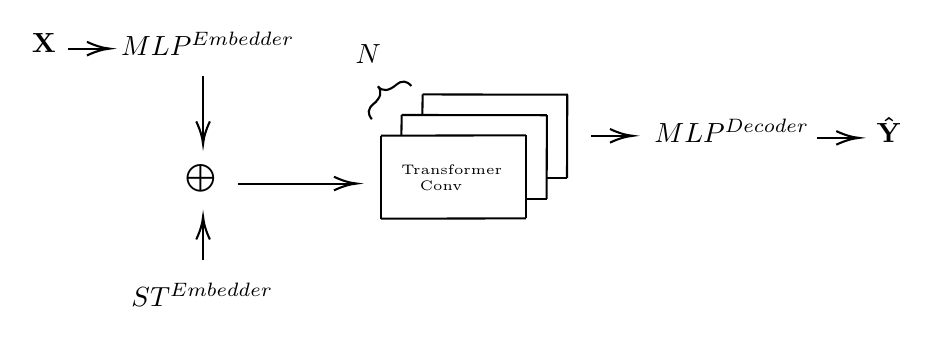
\begin{tikzpicture}[x=0.75pt,y=0.75pt,yscale=-1,xscale=1]
%uncomment if require: \path (0,300); %set diagram left start at 0, and has height of 300

%Shape: Brace [id:dp7019805664018027] 
\draw   (306.33,91) .. controls (304.14,88.39) and (301.74,88.19) .. (299.13,90.38) -- (299.13,90.38) .. controls (295.4,93.52) and (292.44,93.79) .. (290.25,91.18) .. controls (292.44,93.79) and (291.68,96.66) .. (287.95,99.79)(289.63,98.38) -- (287.95,99.79) .. controls (285.34,101.99) and (285.14,104.39) .. (287.33,107) ;
%Straight Lines [id:da24344825121139568] 
\draw    (291.63,114.92) -- (291.63,154.92) ;
%Straight Lines [id:da6110561454804792] 
\draw    (361.7,114.78) -- (361.7,154.78) ;
%Straight Lines [id:da03871795486024654] 
\draw    (291.63,114.92) -- (361.7,114.78) ;
%Straight Lines [id:da49608827752120055] 
\draw    (291.63,154.92) -- (361.7,154.78) ;
%Straight Lines [id:da27192408985546146] 
\draw    (301.69,104.96) -- (371.66,105.08) ;
%Straight Lines [id:da3480819733752343] 
\draw    (301.69,104.96) -- (301.55,114.87) ;
%Straight Lines [id:da3901687935554585] 
\draw    (311.79,95.06) -- (381.76,95.19) ;
%Straight Lines [id:da39197446094452226] 
\draw    (311.79,95.06) -- (311.66,104.98) ;
%Straight Lines [id:da01971233582821519] 
\draw    (371.52,145.35) -- (361.61,145.35) ;
%Straight Lines [id:da8552790800436195] 
\draw    (381.34,135.41) -- (371.43,135.41) ;
%Straight Lines [id:da901598531956911] 
\draw    (371.66,105.08) -- (371.52,145.35) ;
%Straight Lines [id:da7619590199519597] 
\draw    (381.48,95.15) -- (381.34,135.41) ;
%Straight Lines [id:da4912374544292687] 
\draw    (206,175) -- (206,156) ;
\draw [shift={(206,154)}, rotate = 90] [color={rgb, 255:red, 0; green, 0; blue, 0 }  ][line width=0.75]    (10.93,-3.29) .. controls (6.95,-1.4) and (3.31,-0.3) .. (0,0) .. controls (3.31,0.3) and (6.95,1.4) .. (10.93,3.29)   ;
%Straight Lines [id:da3870027998568446] 
\draw    (206,86) -- (206,95) -- (206,117) ;
\draw [shift={(206,119)}, rotate = 270] [color={rgb, 255:red, 0; green, 0; blue, 0 }  ][line width=0.75]    (10.93,-3.29) .. controls (6.95,-1.4) and (3.31,-0.3) .. (0,0) .. controls (3.31,0.3) and (6.95,1.4) .. (10.93,3.29)   ;
%Straight Lines [id:da11332935167733671] 
\draw    (223,138) -- (278,138) ;
\draw [shift={(280,138)}, rotate = 180] [color={rgb, 255:red, 0; green, 0; blue, 0 }  ][line width=0.75]    (10.93,-3.29) .. controls (6.95,-1.4) and (3.31,-0.3) .. (0,0) .. controls (3.31,0.3) and (6.95,1.4) .. (10.93,3.29)   ;
%Straight Lines [id:da8643445648605664] 
\draw    (141,73) -- (159,73) ;
\draw [shift={(161,73)}, rotate = 180] [color={rgb, 255:red, 0; green, 0; blue, 0 }  ][line width=0.75]    (10.93,-3.29) .. controls (6.95,-1.4) and (3.31,-0.3) .. (0,0) .. controls (3.31,0.3) and (6.95,1.4) .. (10.93,3.29)   ;
%Straight Lines [id:da10221146771541123] 
\draw    (502,116) -- (520,116) ;
\draw [shift={(522,116)}, rotate = 180] [color={rgb, 255:red, 0; green, 0; blue, 0 }  ][line width=0.75]    (10.93,-3.29) .. controls (6.95,-1.4) and (3.31,-0.3) .. (0,0) .. controls (3.31,0.3) and (6.95,1.4) .. (10.93,3.29)   ;
%Straight Lines [id:da5913843902335524] 
\draw    (393,115) -- (411,115) ;
\draw [shift={(413,115)}, rotate = 180] [color={rgb, 255:red, 0; green, 0; blue, 0 }  ][line width=0.75]    (10.93,-3.29) .. controls (6.95,-1.4) and (3.31,-0.3) .. (0,0) .. controls (3.31,0.3) and (6.95,1.4) .. (10.93,3.29)   ;

% Text Node
\draw (300,124) node [anchor=north west][inner sep=0.75pt]  [font=\tiny] [align=left] {\begin{minipage}[lt]{28.82pt}\setlength\topsep{0pt}
\begin{center}
{\tiny Transformer }\\{\tiny Conv}
\end{center}

\end{minipage}};
% Text Node
\draw (278,69.4) node [anchor=north west][inner sep=0.75pt]    {$N$};
% Text Node
\draw (170,184.4) node [anchor=north west][inner sep=0.75pt]    {$ST^{Embedder}$};
% Text Node
\draw (165,63.4) node [anchor=north west][inner sep=0.75pt]    {$MLP^{Embedder}$};
% Text Node
\draw (422,105.4) node [anchor=north west][inner sep=0.75pt]    {$MLP^{Decoder}$};
% Text Node
\draw (196,127.4) node [anchor=north west][inner sep=0.75pt]    {$\bigoplus $};
% Text Node
\draw (122,64.4) node [anchor=north west][inner sep=0.75pt]    {$\mathbf{X}$};
% Text Node
\draw (529,104.4) node [anchor=north west][inner sep=0.75pt]    {$\mathbf{\hat{Y}}$};


\end{tikzpicture}


    \caption{Architecture overview}
    \label{fig:architecture}
\end{figure}